\section{Sentence generation as planning}
\label{sec:crisp}


\subsection{Sentence generation with tree-adjoining grammars}

We consider a planning domain that comes up in the generation of
natural language sentences. This is a standard problem in
computational linguistics and can be construed as follows.


\begin{figure}
  \centering
  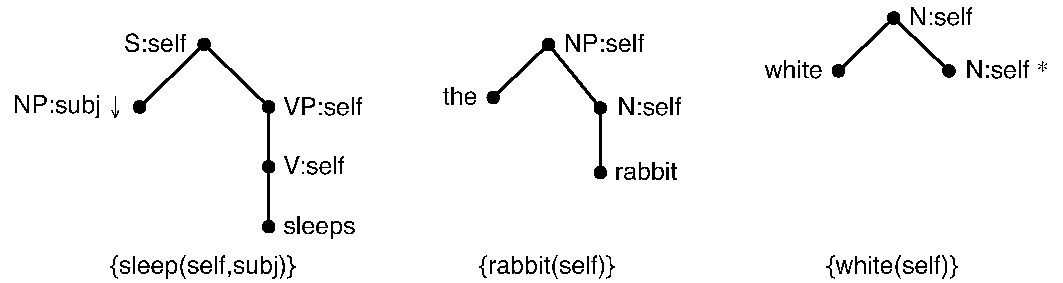
\includegraphics[width=0.75\columnwidth]{pic-grammar}
  \caption{An example grammar in the sentence generation domain.}
  \label{fig:white-rabbit-sleeps-grammar}
\end{figure}

\begin{figure}
  \centering
  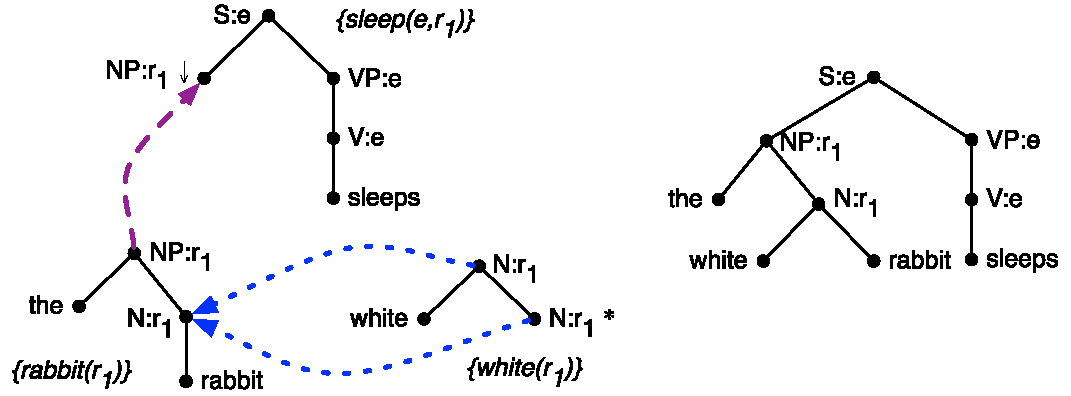
\includegraphics[width=0.75\columnwidth]{pic-derivation}
  \caption{Derivation of ``The white rabbit sleeps.''}
  \label{fig:white-rabbit-sleeps-deriv}
\end{figure}

We assume a tree-adjoining grammar (TAG; \cite{joshi;etal1997}), which
consists of a finite set of \emph{elementary trees} as shown in
Fig.~\ref{fig:white-rabbit-sleeps-grammar}. Elementary trees can be
combined using the operations of \emph{substitution} and
\emph{adjunction}, which are illustrated in
Fig.~\ref{fig:white-rabbit-sleeps-deriv}. Substitution replaces a
substitution node (marked with a downarrow) by a subtree whose root
has the same label, whereas adjunction splits a node in two and
replaces it with a subtree whose root and foot node (marked with an
asterisk) have the same label. A TAG derivation starts with a single
substitution node labeled with a start symbol (in the example, S) and
terminates when all leaves of the tree are labeled with words. In this
way, a TAG grammar defines a language of trees, from which we can read
off a language of strings.

To model the sentence generation problem, we equip every elementary
tree with a set of atoms that specify the \emph{semantic
  representation} of the tree \cite{Stone2003a}.  These terms in these
atoms may be \emph{semantic roles}, such as $\mathsf{subj}$ and
$\mathsf{obj}$ indicating the subject and object positions of a verb;
all substitution nodes of an elementary tree must and the other nodes
may be annotated with semantic roles as well.  In an \emph{instance}
of an elementary tree, all semantic roles have been substituted with
constants from the knowledge base.  Now we can assume a TAG grammar
and two finite sets of ground atoms for the knowledge base and the
semantic representation we want to express in a sentence.  The
sentence generation problem is then to compute a correct TAG
derivation using elementary tree instances such that the input
semantic representation is covered by the semantic representations of
the tree instances; that is, the derivation expresses the intended
meaning.  Furthermore, the assignment of constants to the semantic
roles of the elementary trees must be \emph{unique}: If we replace
each semantic role of every elementary tree in the derivation by a
different variable, there must be exactly one variable assignment that
makes the combined semantic representations of the elementary trees a
subset of the knowledge base.  This ensures that the hearer can
uniquely understand each referring expression.

For example, assume the grammar in
Fig.~\ref{fig:white-rabbit-sleeps-grammar} and a knowledge base that
contains the atoms $\{\mathsf{sleep}(e,r_1), \mathsf{rabbit}(r_1),
\mathsf{rabbit}(r_2), \mathsf{white}(r_1), \mathsf{rabbit}(r_2)\}$,
and let's say we want to express the semantic representation
$\{\mathsf{sleep}(e,r_1)\}$.  Then the derivation in
Fig.~\ref{fig:white-rabbit-sleeps-deriv} would be a correct output of
a sentence generator.  Notice that a derivation for the sentence ``the
rabbit sleeps'' would not be a correct result because the expression
``the rabbit'' is not a unique description of $r_1$: the set
$\{\mathsf{sleep}(x,y), \mathsf{rabbit}(y)\}$ can also be mapped into
the knowledge base by substituting $r_2$ for $y$, so the hearer might
misunderstand the subject as $r_2$. We call $r_2$ a \emph{distractor}
of the referring expression.  Note also that the input semantic
representation did not specify that we should refer to $r_1$ as
``white'' or ``rabbit''; this decision was made by the generation
algorithm.



\subsection{Sentence generation as a planning problem}

The TAG sentence generation problem can be encoded as a planning
problem \cite{KolSto07}.  The key idea is that each operator encodes
the addition of an elementary tree to the derivation; the syntactic
and semantic requirements and effects of doing this are captured in
the operator's precondition and effect.

\begin{figure}
\centering
\begin{minipage}{0.8\textwidth}
{\small%
\begin{verbatim}
(:action sleeps
   :parameters (?u - node  ?subjnode - node  ?nextnode - node
                ?xself - individual  ?xsubj - individual)
   :precondition
       (and (subst S ?u)  (referent ?u ?xself)  (sleep ?xself ?xsubj)
            (current ?subjnode) (next ?subjnode ?nextnode)
   :effect 
       (and (not (subst S ?u))  (expressed sleep ?xself ?xsubj)
            (subst NP ?subjnode)  (referent ?subjnode ?xsubj)
            (not (next ?subjnode)) (next ?nextnode)
            (forall (?y - individual)
                (when (not (= ?y ?xself)) (distractor ?subjnode ?y)))))

(:action rabbit
   :parameters (?u - node  ?xself - individual)
   :precondition 
       (and (subst NP ?u)  (referent ?u ?xself)  (rabbit ?xself))
   :effect 
       (and (not (subst NP ?u))  (canadjoin N ?u)
            (forall (?y - individual)
                (when (not (rabbit ?y)) (not (distractor ?u ?y))))))

(:action white
   :parameters (?u - node  ?xself - individual)
   :precondition 
       (and (canadjoin N ?u)  (referent ?u ?xself)  (rabbit ?xself))
   :effect 
       (forall (?y - individual)
           (when (not (white ?y)) (not (distractor ?u ?y)))))
\end{verbatim}}%
\end{minipage}
\caption{PDDL actions for generating the sentence ``The white rabbit
sleeps.''}
\label{fig:white-rabbit-as-planning}
\end{figure}

More precisely, each operator has a parameter \verb|?u| representing
the syntax node into which the elementary tree is substituted or
adjoined and a parameter \verb|?xR| for each semantic role \verb|R| of
the elementary tree which will be instantiated with the constants with
which the role gets instantiated in the derivation. Furthermore, if
the tree has substitution nodes, there are parameters \verb|?Rnode|
for each role representing these nodes, and an extra parameter
\verb|?nextnode|. The state encodes a list of possible node names;
$\mathsf{current}(n_i)$ expresses that $n_i$ is the next node name
that should be picked when a new substitution node is created, and
$\mathsf{next}(n_i,n_{i+1})$ says that the next node after $n_i$ is
$n_{i+1}$. The atom $\mathsf{subst}(A,u)$ expresses that we need to
still substitute something into the substitution node $u$ with label
$A$; the initial state contains an atom
$\mathsf{subst}(A,\mathsf{root})$ where $\mathsf{root}$ is an
arbitrary name for the root of the derivation.  The values of the
semantic roles are maintained using the $\mathsf{referent}$ atoms.
Finally, we keep track of the uniqueness of referring expressions in
the $\mathsf{distractor}$ atoms: $\mathsf{distractor}(u,a)$ expresses
that the expression at syntax node $u$ could still be misunderstood as
$a$.

The example generation problem above translates into a planning
problem whose domain is shown, in PDDL format, in
Fig.~\ref{fig:white-rabbit-as-planning}. The initial state of the
problem encodes the generation problem's knowledge base; it contains
atoms $\mathsf{rabbit}(r_1)$, $\mathsf{sleep}(e,r_1)$, etc.
Furthermore, the initial state expresses the beginning of the
derivation in atoms $\mathsf{subst}(S,\mathsf{root})$ and
$\mathsf{referent}(\mathsf{root},e)$.  The goal requires syntactic
completeness as $\forall u \forall A \neg \mathsf{subst}(A,u)$ and
unique reference as $\forall u \forall x \neg
\mathsf{distractor}(u,x)$; it also specifies the semantic
representation we want to express in an atom
$\mathsf{expressed}(\mathsf{sleep},e,r_1)$.  A minimal plan for this
problem looks as follows:

\begin{enumerate}
\item $\mathsf{sleeps}(\mathsf{root}, n_1, n_2, e, r_1)$
\item $\mathsf{rabbit}(n_1, r_1)$
\item $\mathsf{white}(n_1, r_1)$
\end{enumerate}

This plan can be automatically decoded into the derivation shown in
Fig.~\ref{fig:white-rabbit-sleeps-deriv}.  The analogous plan with
$r_2$ instead of $r_1$ is not correct because the $\mathsf{sleep}$
precondition of the $\mathsf{sleeps}$ operator is not satisfied.  The
first two steps of the plan alone would not be a correct plan because
they leave an atom $\mathsf{distractor}(n_1, r_2)$ in the state, which
contradicts the goal that all distractors have been eliminated.






%%% Local Variables: 
%%% mode: latex
%%% TeX-master: "main"
%%% End: 
